\chapter{优化问题的定义与基本性质}
\label{chap:optimization}

本章从一个贯穿全书的任务开始：给定带正则项的最小二乘
\begin{equation}
\begin{aligned}
  F(\bm{w})
  &=\frac{1}{2n}\lVert \bm{X}\bm{w}-\bm{y}\rVert_2^2
   +\frac{\lambda}{2}\lVert\bm{w}\rVert_2^2,\\
  \bm{X}&\in\mathbb{R}^{n\times d},\quad
  \bm{w}\in\mathbb R^d,\ \bm y\in\mathbb R^n,\
  \lambda\geq 0,\ n\geq1,
\end{aligned}
  \label{eq:opt-regularized-least-squares}
  % 保留内容迁移前的语义标签，指向同一公式。
\begingroup
\makeatletter
\let\label\ltx@label
\label{eq:prelim-regularized-least-squares}
\endgroup
\end{equation}
其中矩阵$\bm X$的第$i$行为预测输入$\bm x_i^\top$，$\bm y=(y_1,\ldots,y_n)^\top$为观测值。第一项汇总预测与观测之间的平方误差，正则项通过计价的方式改变允许候选之间的比较；若再加上资源限制
\begin{equation}
  \bm{A}\bm{w}=\bm{b},\qquad
  \bm{G}\bm{w}\leq\bm{h},
  \label{eq:opt-linear-resource-constraints}
\end{equation}
约束改变的则是哪些候选可以采用。三者承担的职责不同，后续章节会看到这种区别怎样改变求解方式。

“找一个梯度小的点”并没有回答全部问题：最优值是否真的由某个可行点取得？参数是否唯一？局部信息能推出多强的全局结论？本章按三条线索组织：10.1节先把问题写完整，规定变量、可行域、目标和误差对象；10.2节只用极限与可行域性质证明最优解存在；10.3节再增加凸性与曲率条件，把局部比较提升为全局最优、唯一性和定量误差界。本章不介绍任何迭代算法；怎样产生候选序列是第11章以后的任务。

\section{优化问题与解}
\label{sec:opt-problem-and-solutions}
\label{sec:opt-error-objects}

本节建立后文共用的语言：问题规格确定比较对象，解的定义确定比较范围，误差标准确定停止判断，扩展实值形式则为后面的复合子问题提供统一表达。

\subsection{变量、可行域与最优值}

\subsubsection{优化问题的完整约定}

把一个实际任务写成优化问题，本质上是作四项约定：哪些量可以调整（变量），这些量允许取什么值（可行域），按什么准则比较两个候选（目标函数），以及要求真正达到最优还是只需足够接近。这一步回答的是“机器到底被允许做什么、又按什么打分”。训练模型时，变量通常是模型参数，可行域是满足预算或非负等约束的参数集合，比较准则则是样本损失平均值与正则项之和。

四项约定中任何一项改变，答案都可能改变。同样是“让误差小”：可行域写成整个空间，最优参数可能无界；限制在某个有界集合内，答案就落在集合中；把平方误差换成绝对误差，最优点也可能移动。因此一个优化问题必须同时给出目标函数、变量和可行域：
\[
  \min_{\bm{w}\in C}F(\bm{w}),\qquad
  C=\{\bm{w}\in\mathbb{R}^d:
  \bm{A}\bm{w}=\bm{b},\ \bm{G}\bm{w}\leq\bm{h}\}.
\]
变量$\bm w$是待选择的参数，目标$F$规定怎样比较候选，可行域$C$规定哪些候选允许采用。若等式有$m$条、不等式有$p$条，则$\bm A\in\mathbb R^{m\times d}$、$\bm b\in\mathbb R^m$、$\bm G\in\mathbb R^{p\times d}$、$\bm h\in\mathbb R^p$，向量不等式逐坐标理解。

\subsubsection{可行、下有界与下确界达到}

先固定目标在可行点上为实值：$C$非空时$F:C\to\mathbb R$。问题可能没有合格答案。若$C=\varnothing$，问题\term{不可行}（infeasible），约定其最优值为$+\infty$；若$C\neq\varnothing$但$\inf_{\bm w\in C}F(\bm w)=-\infty$，问题\term{无下界}（unbounded below），最优值为$-\infty$。因此最优值一般是扩展实数；只有可行且下有界时它才是有限实数。例如同时要求$x\leq0$与$x\geq1$不可行；在实线上最小化$x$无下界；而$\inf_{x\in\mathbb R}e^x=0$有有限下界，却没有最小点。

最优值是数
\[
  F^\star=\inf_{\bm w\in C}F(\bm w),
\]
最优解集合是$\argmin_{\bm w\in C}F$，后者可以为空、为单点或包含多个点。写下$\min_C F$只表示提出了求最小值的任务，并不代替存在性证明；声称某个数等于$\min_C F$，才包含“它被可行点取得”的主张。下确界达到与达不到的差别在边界上最清楚：固定同一个目标$x$，在$[0,1]$和$(0,1]$上的下确界都是$0$，但前者由$w=0$取得，后者没有点取得——缺口正在于可行边界是否保留。报告结果时应把“最优值是多少”和“是否有可行点取得它”分开说。

\subsection{解的层次与误差对象}

\subsubsection{全局解、局部解与驻点}

\begin{definition}[全局解、局部解与无约束驻点]
\label{def:opt-solutions-stationarity}
设$C\subseteq\mathbb R^d$非空，$F:C\to\mathbb R$。\term{全局最优解}（global minimizer）$\bm{w}^{\star}\in C$满足
$F(\bm{w}^{\star})\leq F(\bm{w})$对所有$\bm{w}\in C$成立。\term{局部最优解}
（local minimizer）要求存在$r>0$，使该不等式对所有
$\bm w\in C\cap B(\bm w^\star,r)$成立。
无约束可微问题的\term{驻点}（stationary point）满足
$\nabla F(\bm{w})=\bm{0}$。
\end{definition}

全局解与所有可行点比较，局部解只与某个欧氏球内的可行点比较；把邻域写成$C\cap B(\bm w^\star,r)$，边界点的相对比较就包含在定义里。在无约束、候选为定义域内点且目标可微时，多元微积分的一阶必要条件给出$\nabla F(\bm w)=0$。但驻点只消除一阶变化，它可能是极小点、极大点，或鞍点；一般约束问题的最优点还可能有非零梯度，其方向条件要等到第13章。

\subsubsection{误差对象与近似标准}

\paragraph{目标差与一阶残差}

“足够好”有不同的衡量标准。给定$\varepsilon>0$和可行候选$\widehat{\bm w}\in C$，若
\[
  F(\widehat{\bm{w}})-F^\star\leq\varepsilon,
\]
就称$\widehat{\bm w}$为目标值意义下的$\varepsilon$近似解；对无约束可微问题，另一种常见标准是$\lVert\nabla F(\widehat{\bm{w}})\rVert_2\leq\varepsilon$。两者共用一个容差符号并不等价：前者比较全局目标值，后者测量当前位置的一阶残差。

取$f(x)=10^{-8}x^2/2$、$x=10^6$，逐项算出梯度只有$0.01$，目标值却比最小值高$5000$，到最小点$0$的距离仍是$10^6$。平坦方向把一阶变化压得很小，所以小梯度首先回答的只是“局部变化够不够小”。梯度何时能控制目标差、目标差何时能控制距离，都需要额外的曲率常数，将在10.3节和第11章建立。

\paragraph{参数距离与样本预测误差}

评价同一个近似参数，还可以关心三件彼此不同的事。暂取$C=\mathbb R^d$、不加资源约束，以式~\eqref{eq:opt-regularized-least-squares}为目标，选定一个最小点$\bm w^\star$，则
\[
  F(\widehat{\bm{w}})-F^\star,\qquad
  \lVert\widehat{\bm{w}}-\bm{w}^\star\rVert_2,\qquad
  \frac{1}{\sqrt n}\lVert\bm X(\widehat{\bm{w}}-\bm{w}^\star)\rVert_2
\]
分别是目标值误差、参数误差和在给定样本输入上的均方根预测误差。预测误差只针对给定输入，不自动代表未知输入上的表现；最小点不唯一时，参数误差还需指定参照解，或改成到最小点集合的距离。

例如$n=1$、$\bm x_1=(1,0)^\top$、$y_1=0$、$\lambda=0$时，目标为$F(w_1,w_2)=w_1^2/2$。参照解$(0,0)$与参数$(0,100)$的目标值都为$0$，样本预测也相同，参数距离却是$100$。差别的根源在于目标和当前观测都没有约束第二个坐标；把目标误差算得再精确，也补不回该方向缺失的信息。

\subsection{扩展实值目标与约束指标}

若希望在同一个目标式里既比较代价、又排除不可行点，可以约定不可行点的代价为$+\infty$。

\begin{definition}[适当函数、有效定义域与约束指标]
\label{def:opt-proper-domain-indicator}
函数$f:\mathbb R^d\to\mathbb R\cup\{+\infty\}$若不恒为$+\infty$，称为适当函数；
它从不取$-\infty$。其\term{有效定义域}（effective domain）为
$\operatorname{dom}f=\{\bm x:f(\bm x)<+\infty\}$。
集合$C$的扩展实值指标函数为$\iota_C(\bm x)=0$（$\bm x\in C$），在其余点取$+\infty$。
\end{definition}

在$C$非空、$F$为$C$上实值函数的设定下，受约束任务与$F+\iota_C$的有限值候选及其取值逐点对应，所以两者下确界相同，且在有限最优值达到时最小点相同；这里用下确界表述，不预设达到。若$C=\varnothing$，组合目标没有有限值候选、不适当，应报告不可行，不能把全部取$+\infty$的点当作可用最优解。它也不同于取值$0,1$的集合指示函数$\mathbb I\{\cdot\}$：有限惩罚只是“不喜欢”违规候选，$\iota_C$才真正把违规点排除出最小化。这种统一写法使后面的非光滑子问题和约束子问题不必另备一套符号。

\section{最优解的存在}
\label{sec:opt-existence}

下确界只保证可以任意逼近，不保证达到。讨论怎样求解之前，先确认所求对象存在；这一构造甚至不需要算法。当$m=\inf_C F$有限时，可以逐项选取$F(\bm w^{(k)})\leq m+1/k$；若下确界为$-\infty$，则逐项要求$F(\bm w^{(k)})\leq-k$。这样选出的序列称为最小化序列。但“目标值越来越低”与“参数有收敛子列”是两回事，从序列走到最小点必须补齐三个环节：序列有收敛子列，极限仍可行，目标值的比较能传到极限。$e^{-x}$沿$x_k=k$目标值趋于下确界$0$，参数却逃向无穷远，第一个环节就失败；开区间边界上则可能失败在第二个环节。

\subsection{紧域上的连续目标}

若$C\subseteq\mathbb R^d$非空、闭且有界（即紧），$F:C\to\mathbb R$连续，则有限维紧性让最小化序列有域内收敛子列，连续性把其目标值的极限传给极限点。这就是多元微积分章建立的极值存在结论：$F$在$C$上达到全局最小值，这里直接复用，不重做一般紧致理论。对有界闭资源集合，只要确认非空，连续拟合目标便达到最小值；若可行域无界，这条论证就缺少序列的有界性，需要下一小节用目标本身把序列拦住，但这并不意味着无界可行域必无解。

\subsection{紧下水平集上的下半连续目标}

\paragraph{下半连续与闭下水平集}

存在性证明需要的不是连续函数的等式，而是更弱的单向条件。

\begin{definition}[强制性与下半连续性]
\label{def:opt-coercive-lower-semicontinuous}
设$C\subseteq\mathbb R^d$，$F:C\to(-\infty,+\infty]$。若沿$C$中的任意序列，
$\lVert\bm{w}\rVert_2\to\infty$时$F(\bm{w})\to+\infty$，称$F$是
\term{强制的}（coercive）。$F$在$C$上\term{下半连续}
（lower semicontinuous）要求对每个收敛序列
$\bm{w}^{(k)}\to\bm{w}$（序列与极限点均属于$C$）都有
\[
  F(\bm{w})\leq\liminf_{k\to\infty}F(\bm{w}^{(k)}).
\]
\end{definition}

下半连续允许函数值在极限点向下跳，却不允许它突然高于邻近值的下极限。等价地，每个下水平集$\{\bm w\in C:F(\bm w)\leq a\}$在$C$的相对拓扑中都是闭集：若其中有序列收敛，下半连续性保证极限仍落在该水平集内；反过来，违反下半连续时也能选出一个被极限越过的水平。注意相对闭还要与$C$本身的闭性合用，才能把它当作环境欧氏空间中的闭集。

\paragraph{强制性阻止序列逃向无穷远}

强制性规定参数趋于无穷时代价趋于无穷。用反证即可看到它的作用：若某个有限下水平集无界，就能从中选出范数趋于无穷、目标却不超过同一有限水平的序列，与强制性矛盾。因此强制性保证每个有限下水平集有界，给最小化序列提供“留在有界区域”的依据；它不是存在最小点的必要条件，只是无界域上取得有界性的一种充分来源。

\paragraph{在闭下水平集上取得最小值}

下面把三个条件各管一段拼成完整论证。设$C$非空且闭，$F:C\to(-\infty,+\infty]$适当、下半连续并强制。取$\bar{\bm w}\in C$使$F(\bar{\bm w})<+\infty$，考虑
\[
  K=\{\bm{w}\in C:F(\bm{w})\leq F(\bar{\bm{w}})\}.
\]
若$\inf_C F=F(\bar{\bm w})$，则$\bar{\bm w}$已是最小点；否则任一最小化序列从某项起都落入$K$，只保留这段尾序列即可。强制性使$K$有界，下半连续性与$C$的闭性使$K$闭，故$K$在有限维空间中紧。该尾序列有子列收敛到$\bm w^\star\in K$，下半连续性给出
\[
  F(\bm w^\star)\leq\liminf_kF(\bm w^{(k)})=\inf_C F,
\]
与下确界的反向不等式合成等号，下确界因而达到。若事先假设下确界为$-\infty$，同一不等式会迫使$F(\bm w^\star)=-\infty$，与适当性矛盾，所以这些条件也排除了无下界情形。

图~\ref{fig:vol1-add-coercive-sublevels}把“留在有界区域”和“逃向无穷远”并排呈现。
\begin{figure}[!htb]
  \centering
  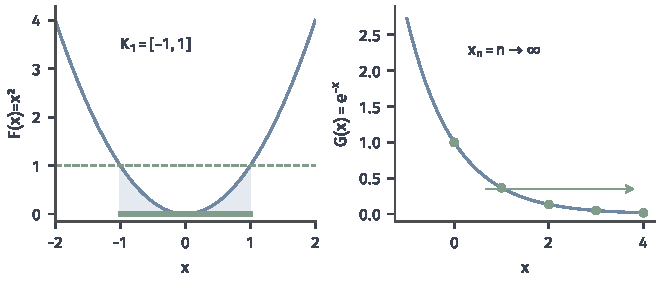
\includegraphics[width=112mm]{figures/01-mathematical-preliminaries-upper/01-mathematical-language-combinatorics-analysis-optimization/matplotlib/comprehension-additions/coercive-sublevels.pdf}
  \caption{全实线上的两个连续目标。左图$F(x)=x^2$的下水平集$K_1=\{x:F(x)\leq1\}=[-1,1]$有界；右图$G(x)=e^{-x}$沿$x_n=n$趋近下确界$0$，但没有最小点。左侧浅色仅标出下水平范围内的函数图下区域，绿线才表示参数集合$K_1$。这组例子说明存在性条件的职责，不声称强制性是任何最小点存在的必要条件。}
  \label{fig:vol1-add-coercive-sublevels}
\end{figure}

\noindent\begin{minipage}{\linewidth}
回到最小二乘：当$\lambda>0$时$F(\bm w)\geq\lambda\lVert\bm w\rVert_2^2/2$，在非空闭资源域上下水平集有界，故最小点存在。逐项回看各条件的职责：强制性留住有界性，闭域留住可行极限，下半连续把目标比较传到极限。它们都是充分条件；下一节增加的凸性仍须另行核验。

\section{凸性条件下的最优解性质}
\label{sec:opt-convexity}

存在性只回答“有没有”。本节依次加强三个条件：凸性把局部最优提升为全局最优，严格凸性排除多个最小点，强凸性再给出统一的曲率下界，把目标值差换算成参数距离。三者逐层增强，不能互相替代。

\subsection{凸性与全局最优}

\subsubsection{凸集、凸组合与凸函数}

\paragraph{远处更优点怎样影响局部比较}

局部最优只和附近候选比较。设想地形中有两个互相隔开的山谷：站在其中一个谷底向四周看，处处都更高，局部上已经最优，但另一个山谷可能更低，而局部信息里没有远处山谷的任何线索。如果任意两个可行点之间的线段都仍在可行域内，且沿这条线段的目标值不超过两端值的加权平均，那么远处一旦有更低的点，连向它的线段就会在当前点附近给出一个更低的点，“假谷底”随即被排除。这两项条件分别是集合与函数的凸性。
\end{minipage}\par
\begin{definition}[凸集与凸函数]
\label{def:opt-convex-set-function}
集合$C\subseteq\mathbb R^d$为\term{凸集}（convex set），是指对任意
$\bm{u},\bm{v}\in C$和$\theta\in[0,1]$，
$\theta\bm{u}+(1-\theta)\bm{v}\in C$。
定义在凸集$C$上的函数$f:C\to\mathbb R$若对任意$\bm u,\bm v\in C$和$\theta\in[0,1]$满足
\begin{equation}
  f(\theta\bm{u}+(1-\theta)\bm{v})
  \leq
  \theta f(\bm{u})+(1-\theta)f(\bm{v}),
  \label{eq:opt-convex-function}
\end{equation}
就称为\term{凸函数}（convex function）。若$-f$凸，则称$f$凹。
\end{definition}
线性等式、线性不等式和范数球的解集都是凸集，交集仍为凸集，所以式~\eqref{eq:opt-linear-resource-constraints}定义凸可行域。式~\eqref{eq:opt-convex-function}右侧是两个函数值的\term{加权平均}（weighted average）：两个系数非负且和为$1$，分别规定两端点值在平均中所占的份额。

\paragraph{有限凸组合、凸包与Jensen不等式}

二点线段可以反复使用。对非空集合$A\subseteq\mathbb R^d$中的有限个点$\bm a_1,\ldots,\bm a_m$，称
\[
  \sum_{i=1}^m\alpha_i\bm a_i,\qquad
  \alpha_i\geq0,\quad \sum_{i=1}^m\alpha_i=1
\]
为它们的凸组合；所有有限凸组合组成的集合记为$\operatorname{conv}(A)$。把“凸组合的凸组合”展开并合并权重，新权重仍非负且和为$1$，故$\operatorname{conv}(A)$凸；而任何包含$A$的凸集由二点组合归纳都包含全部有限凸组合，所以$\operatorname{conv}(A)$是包含$A$的最小凸集，即$A$的凸包。当$A$有限时，系数集合是闭有界的，线性加权映射连续，其像$\operatorname{conv}(A)$紧。凸包不默认闭：$A=(0,1)$的凸包仍是开区间$(0,1)$；若要把可逼近的极限也纳入，取闭凸包$\overline{\operatorname{conv}(A)}$，它是包含$A$的最小闭凸集。这两个对象将在松弛和梯度凸包投影中使用。

对凸域内的有限个点与凸函数，从二点凸性归纳得到\term{Jensen不等式}（Jensen's inequality）：
\begin{equation}
  f\left(\sum_{i=1}^m\alpha_i\bm{w}_i\right)
  \leq\sum_{i=1}^m\alpha_i f(\bm{w}_i).
  \label{eq:opt-jensen}
\end{equation}
归纳时先把前$m-1$个点的权重按$1-\alpha_m$归一化成一个加权平均，再与第$m$个点应用二点凸性；$\alpha_m=1$时直接是末点等式，避免除以零。非负与归一化不是装饰：允许负权重后组合点可能落到凸包之外，不等式不再有保证。

对扩展实值目标，式~\eqref{eq:opt-convex-function}只在有限取值的点上检验，并要求有效定义域凸，以免出现$0\cdot(+\infty)$的无意义运算。

\paragraph{扩展实值目标的凸性}

回到10.1节的统一形式：扩展实值凸函数的有效定义域必须凸，凸性不等式在两个端点都取有限值时检验，端点权重为零的情形按有效域约定处理。这里转换的只是函数的取值范围，有限凸组合的几何仍然是共同基础，不引入积分版Jensen。

\subsubsection{可微凸性的判据}

\paragraph{一阶支撑下界}

凸函数图像位于弦下方；可微时，它还位于每点切线的上方。

\begin{theorem}[凸函数的一阶与二阶判据]
\label{thm:opt-convexity-criteria}
设$C$为开凸集。可微函数$f:C\to\mathbb{R}$凸，当且仅当对任意
$\bm{u},\bm{v}\in C$，
\begin{equation}
  f(\bm{v})\geq f(\bm{u})
  +\langle\nabla f(\bm{u}),\bm{v}-\bm{u}\rangle.
  \label{eq:opt-first-order-convexity}
\end{equation}
若$f$二阶可微，则这又等价于
$\nabla^2f(\bm{w})\succeq\bm{0}$对所有$\bm{w}\in C$成立。
\end{theorem}

\begin{proof}
若$f$凸，沿线段令$\phi(t)=f(\bm{u}+t(\bm{v}-\bm{u}))$。由凸性，
$[\phi(t)-\phi(0)]/t\leq\phi(1)-\phi(0)$，令$t\downarrow0$便得
式~\eqref{eq:opt-first-order-convexity}。反过来，令
$\bm{z}=\theta\bm{u}+(1-\theta)\bm{v}$，分别把一阶不等式用于
$(\bm{z},\bm{u})$和$(\bm{z},\bm{v})$，乘以$\theta$与$1-\theta$后相加，
线性项抵消，恢复式~\eqref{eq:opt-convex-function}。

二阶情形：把一阶判据用于$\bm{w}$与$\bm{w}+t\bm{v}$，再对$t$取二阶局部极限，
得$\bm{v}^{\top}\nabla^2f(\bm{w})\bm{v}\geq0$。反之，沿任意线段定义
$\phi(t)$，则
$\phi''(t)=(\bm{v}-\bm{u})^{\top}\nabla^2f(\bm{u}+t(\bm{v}-\bm{u}))
(\bm{v}-\bm{u})\geq0$，一元函数$\phi$凸，故$f$凸。
\end{proof}

判据要求在整个开凸讨论域上成立：单个候选处Hessian半正定不能证明全域凸性，非开的约束域也不能不加说明地套用同样的导数陈述。图~\ref{fig:opt-convex-chord-tangent}把弦上界与切线下界画在一起，二者来自不同的比较对象，不能把某点的切线误当作连接两个函数值的弦\scite{math-boyd2004convex}。
\begin{figure}[htbp]
  \centering
  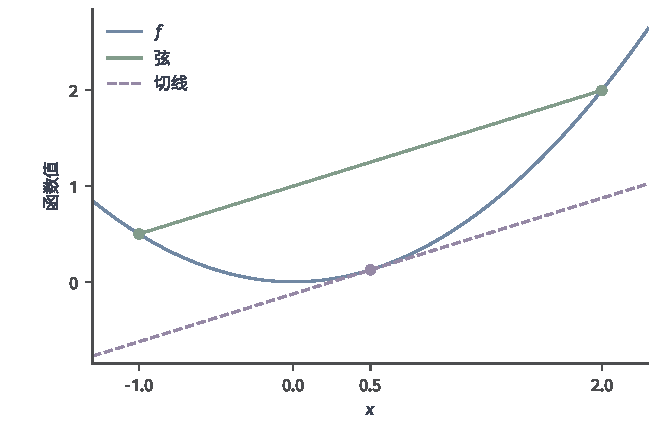
\includegraphics[width=112.0mm]{figures/01-mathematical-preliminaries-upper/01-mathematical-language-combinatorics-analysis-optimization/matplotlib/opt-convex-chord-tangent/figure.pdf}
  \caption{$f(x)=x^2/2$的弦与切线。蓝线为函数，绿线连接$u=-1$与$v=2$的函数值，
 在这两个输入之间给出弦上界；紫虚线是在$x_0=1/2$处的一阶仿射下界，适用于整个实线。
 绿线的上界只在其端点之间使用，切线下界来自凸性。图为解析教学示例。}
 \label{fig:opt-convex-chord-tangent}
\end{figure}

\subsubsection{局部最优与驻点的全局意义}

凸性把局部比较提升为全局比较。设凸域中局部最小点$\bm u$不是全局最小点，取$\bm v\in C$使$f(\bm v)<f(\bm u)$，则对任意$t\in(0,1)$，
\[
  f(\bm u+t(\bm v-\bm u))
  \leq(1-t)f(\bm u)+tf(\bm v)<f(\bm u),
\]
取足够小的$t$，新点仍在局部比较邻域内，与局部最优矛盾。这个证明不要求可微，所以对凸的非光滑目标也成立。对无约束可微凸目标，把$\nabla f(\bm w^\star)=\bm0$代入式~\eqref{eq:opt-first-order-convexity}便得$f(\bm v)\geq f(\bm w^\star)$，因此凸问题的驻点就是全局最小点；反过来，非凸问题找到驻点只能说明附近没有一阶下降方向。边界上的约束最优点并不要求普通梯度为零。

\subsection{严格凸性与解的唯一性}

凸函数可以沿某个方向保持不变，所以“局部即全局”并没有排除多个最小点。最小点不唯一时，返回哪个解取决于算法路径，与最小点距离有关的误差界也无从定义。

\begin{definition}[严格凸函数]
\label{def:opt-strict-convexity}
设$C$凸，$f:C\to\mathbb R$。若式~\eqref{eq:opt-convex-function}对所有
$\bm u\neq\bm v$及$0<\theta<1$严格成立，则称$f$严格凸。
\end{definition}

若两个不同点$\bm u,\bm v$都达到最小值$m$，严格凸性使其中点的函数值严格小于$(m+m)/2=m$，矛盾。因此严格凸只保证最小点至多一个：严格凸函数$e^x$在实线上就没有最小点，存在性仍须交给10.2节合用。反方向也不成立：$|x|$有唯一最小点，但在同号线段上是仿射、并不严格凸，所以不能由解唯一反推严格凸。

回到式~\eqref{eq:opt-regularized-least-squares}：$\lambda=0$且$\bm X$不满列秩时，沿零空间方向目标不变，存在一整条最优线段；$\bm X$满列秩或$\lambda>0$时，任意非零方向$\bm d$都有$\|\bm X\bm d\|_2^2/n+\lambda\|\bm d\|_2^2>0$，目标严格凸。再与闭可行域上的存在性合用，才能断言解唯一。

\subsection{强凸性与误差几何}
\label{sec:opt-strong-convex}

严格凸只要求“中点严格更低”，没有规定低多少：两个严格凸函数可以一个像浅口碗、一个像深漏斗。这个“低多少”决定目标误差能换回多小的参数误差，也决定后面梯度类算法收敛得多快。强凸性要求弦段与函数之间至少留出一个与距离平方成比例的间隔。它是目标自身的误差几何，尚不涉及算法的迭代速度。

\subsubsection{相对于范数的统一曲率下界}

\begin{definition}[相对于范数的强凸性]
\label{def:opt-strong-convexity}
设$C$是实赋范空间中的凸集，$f:C\to\mathbb{R}$，$\mu>0$。若对任意
$\bm{u},\bm{v}\in C$和$\theta\in[0,1]$都有
\begin{equation}
 f(\theta\bm{u}+(1-\theta)\bm{v})
 \leq\theta f(\bm{u})+(1-\theta)f(\bm{v})
 -\frac{\mu}{2}\theta(1-\theta)\lVert\bm{u}-\bm{v}\rVert^2,
 \label{eq:opt-norm-strong-convexity}
\end{equation}
则称$f$相对于$\lVert\cdot\rVert$是\term{$\mu$强凸}（$\mu$-strongly convex）的。
\end{definition}

这个定义可以容纳非光滑正则项和欧氏范数以外的范数：$|x|+\mu x^2/2$虽在$0$处不可微，仍相对于绝对值范数$\mu$强凸——绝对值部分提供凸性，二次部分恰好补上式~\eqref{eq:opt-norm-strong-convexity}中的距离平方间隔。而$x^4$严格凸，却在原点曲率为零、给不出全域统一的二次下界，说明强凸增加的是定量条件。

在欧氏空间的开凸集上，若$f$可微，对$f-\mu\|\cdot\|_2^2/2$应用凸性判据，强凸性等价于
\begin{equation}
  f(\bm{v})\geq f(\bm{u})+
  \langle\nabla f(\bm{u}),\bm{v}-\bm{u}\rangle
  +\frac{\mu}{2}\lVert\bm{v}-\bm{u}\rVert_2^2;
  \label{eq:opt-first-order-strong-convexity}
\end{equation}
二阶可微时又等价于$\nabla^2f(\bm w)\succeq\mu\bm I$。一般范数的平方未必是欧氏二次型，所以不能把Hessian写法当作所有范数下的通用定义。对最小二乘可直接读出Hessian为$\bm X^\top\bm X/n+\lambda\bm I$：$\lambda>0$时目标至少$\lambda$强凸；秩亏且无正则时仍凸，却取不到正的强凸常数。

\subsubsection{目标差控制到最小点的距离}

设凸域中最小点$\bm w^\star$已存在。把强凸定义用于$\bm w^\star$与任意可行$\bm w$，并用最优性给线段上的函数值加下界：对任意$t\in(0,1)$，
\[
 f(\bm w^\star)\leq(1-t)f(\bm w^\star)+tf(\bm w)
 -\frac{\mu}{2}t(1-t)\|\bm w-\bm w^\star\|^2.
\]
除以$t>0$再令$t\downarrow0$，得到
\begin{equation}
 f(\bm w)-f(\bm w^\star)\geq\frac{\mu}{2}\|\bm w-\bm w^\star\|^2,
 \qquad
 \|\bm w-\bm w^\star\|\leq\sqrt{\frac{2(f(\bm w)-f^\star)}{\mu}}.
 \label{eq:opt-strong-convex-distance}
\end{equation}
这同时排除了不同的最小点，并把目标精度换算成参数精度。证明没有假设最优点在内部或目标可微，因此对固定凸域边界上的非光滑强凸目标同样成立；它仍未回答算法取得该目标精度需要多少轮——那是第11章的问题。最优解对问题扰动（线性项变化、约束参数变化）的响应将分别在11.5和13.8讨论。

\section{本章小结}

本章围绕同一个候选区分了五件事：可行性、达到性、全局或局部最优、驻点残差，以及目标差、参数距离、预测差三种误差。存在、唯一和误差大小分别回答不同问题：紧域上连续目标达到最小值，闭域上适当、下半连续且强制的目标通过紧下水平集达到最小值；凸性把局部最优提升为全局最优，严格凸把最小点限制为至多一个，强凸再用统一常数把目标差换算成参数距离。唯一性既不保证数值稳定，也不决定算法速度，指定尺度下的扰动分析要到11.5节。

本章始终没有生成任何迭代序列。下一章起，我们才把局部导数、曲率常数和这里的误差关系放进更新过程：方法说明当前困难、改变的机制和执行步骤，再检验每一步与有限预算下的保证；不能由本章的问题性质直接推断任意算法都能取得相同结果。
